\documentclass[12pt, %
openright,
oneside, %
%twoside, %TCC: Se seu texto tem mais de 100 páginas, descomente esta linha e comente a anterior
a4paper,    %
%english,   %
brazil]{facom-ufu-abntex2}

\usepackage{graphicx}
\usepackage[utf8]{inputenc}
\usepackage[T1]{fontenc}
\usepackage[brazil]{babel}
\usepackage{multirow}
\usepackage{listings}
\usepackage{hyperref}

\autor{William Johnson dos Santos Okano} %TCC
\data{2018}
\orientador{Prof. Dr. André Ricardo Backes} %TCC
%\coorientador{Algum?} %TCC


% ---
% Informações de dados para CAPA e FOLHA DE ROSTO
% ---

\titulo{Implementação de uma biblioteca gráfica cross-platform utilizando OpenGL e GLFW} %TCC

\hypersetup{pdfkeywords={biblioteca}{opengl}{cross-plaftorm}{glfw}} %TCC

\begin{document}
\frenchspacing

% ----------------------------------------------------------
% ELEMENTOS PRÉ-TEXTUAIS
% ----------------------------------------------------------
%\pretextual
\imprimircapa
\imprimirfolhaderosto


% ---
% Inserir folha de aprovação
% ---
%
% \includepdf{folhadeaprovacao_final.pdf} %TCC: depois de aprovado o trabalho, descomente esta linha e comente o próximo bloco para incluir scan da folha de aprovação.
%

\begin{folhadeaprovacao}

  \begin{center}
    {\ABNTEXchapterfont\large\imprimirautor}

    \vspace*{\fill}\vspace*{\fill}
    {\ABNTEXchapterfont\bfseries\Large\imprimirtitulo}
    \vspace*{\fill}

    \hspace{.45\textwidth}
    \begin{minipage}{.5\textwidth}
        \imprimirpreambulo
    \end{minipage}%
    \vspace*{\fill}
   \end{center}

   Trabalho aprovado. \imprimirlocal, 22 de Junho de 2018: %TCC:

   \assinatura{\textbf{\imprimirorientador} \\ Orientador}
   \assinatura{\textbf{Prof. João da Silva}}% \\ Convidado 1} %TCC:
   \assinatura{\textbf{Prof. Maria dos Santos}}% \\ Convidado 2} %TCC:
   %\assinatura{\textbf{Professor} \\ Convidado 3}
   %\assinatura{\textbf{Professor} \\ Convidado 4}

   \begin{center}
    \vspace*{0.5cm}
    {\large\imprimirlocal}
    \par
    {\large\imprimirdata}
    \vspace*{1cm}
  \end{center}

\end{folhadeaprovacao}

% ---


%%As seções dedicatória, agradecimento e epígrafe não são obrigatórias.
%%Só as mantenha se achar pertinente.

% ---
% Dedicatória
% ---
%\begin{dedicatoria}
%   \vspace*{\fill}
%   \centering
%   \noindent
%   \textit{Dedico a \lipsum[10]}  %TCC:
%   \vspace*{\fill}
%\end{dedicatoria}
% ---

% ---
% Agradecimentos
% ---
%\begin{agradecimentos}
%Agradeço a \lipsum[30]. %TCC:
%\end{agradecimentos}
% ---

% ---
% Epígrafe
% ---
%\begin{epigrafe}
%    \vspace*{\fill}
%	\begin{flushright}
%		\textit{``Alguma citação que ache conveniente? \lipsum[10]''} %TCC:
%	\end{flushright}
%\end{epigrafe}
% ---


%\iffalse % Descomentar Resumo no final
\begin{resumo} %TCC:
 Segundo a , o resumo deve ressaltar o
 objetivo, o método, os resultados e as conclusões do documento. A ordem e a extensão
 destes itens dependem do tipo de resumo (informativo ou indicativo) e do
 tratamento que cada item recebe no documento original. O resumo deve ser
 precedido da referência do documento, com exceção do resumo inserido no
 próprio documento. (\ldots) As palavras-chave devem figurar logo abaixo do
 resumo, antecedidas da expressão Palavras-chave:, separadas entre si por
 ponto e finalizadas também por ponto.

 \vspace{\onelineskip}

 \noindent
 \textbf{Palavras-chave}:Biblioteca de funções, elementos gráficos, OpenGL. %TCC:
\end{resumo}
%\fi

% ---
% inserir lista de ilustrações
% ---
\pdfbookmark[0]{\listfigurename}{lof}
\listoffigures*
\cleardoublepage
% ---

\iffalse
% ---
% inserir lista de tabelas
% ---
\pdfbookmark[0]{\listtablename}{lot}
\listoftables*
\cleardoublepage
% ---
\fi


% ---
% inserir lista de abreviaturas e siglas
% ---
\begin{siglas} %TCC:
  \item[GLFW] \textit{OpenGL FrameWork}
  \item[API] \textit{Application Programming Interface}
  \item[RGB] \textit{Red, Green and Blue}
  \item[FPS] \textit{Frame por segundo}
  %\item[456] Isto é um número
  %\item[123] Isto é outro número
  %\item[Zézão] este é o meu nome
\end{siglas}
% ---

%% ---
%% inserir lista de símbolos, se for adequado ao trabalho. %TCC:
%% ---
%\begin{simbolos}
%  \item[$ \Gamma $] Letra grega Gama
%  \item[$ \Lambda $] Lambda
%  \item[$ \zeta $] Letra grega minúscula zeta
%  \item[$ \in $] Pertence
%\end{simbolos}
%% ---

% ---
% inserir o sumario
% ---
\pdfbookmark[0]{\contentsname}{toc}
\tableofcontents*
\cleardoublepage
% ---





% ----------------------------------------------------------
% ELEMENTOS TEXTUAIS
% ----------------------------------------------------------
\textual


% ----------------------------------------------------------
% Introdução
% ----------------------------------------------------------

\chapter[Introdução]{Introdução}

Introdução

\section{Objetivos}
Objetivos

\section{Funcionalidades previstas}


\chapter{Trabalhos Correlatos}

\textbf{Falar sobre a lista abaixo. Não definitivo. Falta construir}
\begin{itemize}
    \item Borlang Graphics Interface (BGI)
\end{itemize}

\chapter{Desenvolvimento}

\section{Tecnologias Empregadas}

\subsection{Linguagem de programação C}
A linguagem de programação \citeonline{C:About} foi criada por Dennis MacAlistair Ritchie entre 1969 e 1973 na \citeonline{BellLabs:Site} e trata-se de uma linguagem de propósito geral que pode ser utilizada com os paradigmas imperativo, também conhecido como procedural, e o paradigma estruturado. Segundo o site \citeonline{GeneralPurposeLanguage:About}, uma linguagem de propósito geral é aquela que não é limitada apenas à algum tipo de hardware específico ou para uma aplicação especializada.

A linguagem de programação C foi escolhida por ser uma das linguagens mais utilizadas para o ensino de programação nas universidades brasileiras. Uma pesquisa conduzida online em um grupo de programação chamado \citeonline{TauloPorrens}, um fórum que concentra mais de 71.000 programadores e entusiastas brasileiros, foi obtido um resultado de que aproximadamente 55\% das universidades brasileiras escolhem C como a primeira, ou uma das primeiras, linguagens para o ensino de introdução à programação, como pode-se observar na figura ~\ref{fig:pesquisa_linguagem_tcc}. Isso representa 570 votos em uma pesquisa com 1036 respostas. A linguagem de programação Java, que se sagrou em segundo lugar como mais utilizada, teve apenas 169 votos, representando 16,31\% do total de votos. O resultado para a \citeonline{APDA:EnqueteLinguagem} pode ser encontrada no link \hyperref[https://www.facebook.com/groups/osadpa/permalink/1508699765902212/]{https://www.facebook.com/groups/osadpa/permalink/1508699765902212/}.

Apesar do nome caricato do grupo onde foi conduzida a pesquisa, se trata de um grupo sério sobre programação em geral e é o grupo de encontro para os utilizadores da página Programação Depressão, uma página de comédia com o cotidano de profissionais, e relacionados, à área de Tecnologia da Informação. O grupo A.P.D.A. é o grupo onde se encontram os seguidores da página Programação Depressão. O nome do grupo foi escolhido relacionado ao nome da página.

\pagebreak
\begin{figure}[htbp]
  \centering
  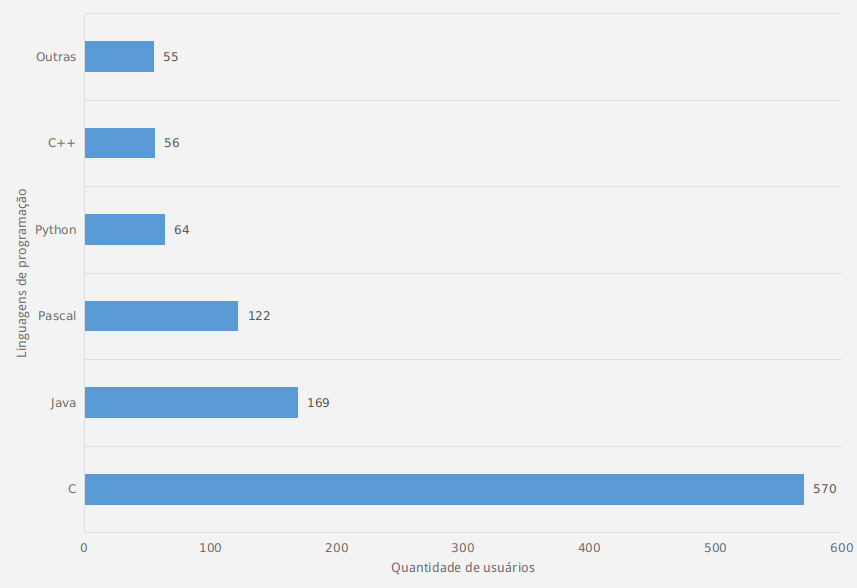
\includegraphics[scale=0.7]{images/pesquisa_linguagem_tcc.png}
  \caption{Linguagens de programação utilizadas primariamente no ensino de introdução à programação}
  \label{fig:pesquisa_linguagem_tcc}
\end{figure}

\subsection{OpenGL}
O \citeonline{OpenGL:About} é uma biblioteca gráfica para desenvolvimento de aplicações interativas. Desde sua introdução, no ano de 1992, a biblioteca OpenGL se tornou  a interface de de programação de aplicação (API) mais utilizada com suporte a 2D e 3D pela indústria. O OpenGL foi escolhido como biblioteca gráfica pela sua qualidade de ser altamente portável estando presente em várias plataformas, como Windows, Linux, Unix, MacOS, e mais. Outro motivo foi também por possuir um bom desempenho e poder ser utilizada em conjunto com várias linguagens de programação, dentre as quais foi escolhida a linguagem de programação \citeonline{C:About}.

A biblioteca gráfica \citeonline{OpenGL:About} foi escolhida em detrimento de outras por ser mais simples, porém versátil, e suas já citadas qualidades: performance, largamente utilizada, interoperável entre plataformas e por ter fácil integração com a linguagem de programação C. Outros fatores que influenciaram a sua escolha foi a vasta documentação, como websites, livros e cursos online. Alguns sites que promovem a documentação de utilização do OpenGL são o próprio site do OpenGL \hyperref[https://opengl.org/]{https://opengl.org/}, o website \citeonline{LearnOpenGL:Site} e o livro OpenGL Programming Guide: The Official Guide to Learning OpenGL, Version 1.2, do autor \citeonline{Woo:1999:OPG:554539}.

A forma que o OpenGL trabalha para renderizar as formas na tela é baseado em uma máquina de estados. Cada item renderizado pelo OpenGL fica num buffer secundário e só é renderizado quando explicitamente solicitado. Ao renderizar o buffer ele então realizar a troca do buffer primário pelo secundário, exibindo assim apenas o quadro renderizado por completo, evitando assim o \textit{tearing}. \textit{Tearing} é o efeito que ocorre quando parte do frame é renderizado utilizando informações antiga, exibindo assim parte do quadro com uma imagem e outra parte com os dados novos.

\subsection{GLFW}
Segundo o site da \citeonline{GLFW:About}, GLFW é uma biblioteca gráfica open-source, multi-plataforma para desenvolvimento desktop utilizando OpenGL, OpenGL ES e Vulkan. Ela é responsável por criar janelas de forma unificada entre diferentes sistemas operacionais, contextos OpenGL e receber entradas de dados e eventos.

A biblioteca GLFW foi escrita em C e possui suporte nativo para Windows, macOS e vários sistemas Unix \cite{Unix:About} que utilizam o sistema de janelas X Window System \cite{X:About}, como por exemplo Linux \cite{Linux:About} e FreeBSD \cite{FreeBSD:About}.

As motivações que levaram a escolha da biblioteca gráfica GLFW foram a criação de janelas de forma transparente entre diversos sistemas operacionais, suporte para OpenGL, suporte a vários monitores e várias janelas simultâneas, suporte para mouse, teclado e joystick, além de ser a biblioteca mais atualizada, tendo vasta documentação e grande comunidade ativa. A documentação completa da biblioteca GLFW pode ser encontrada no website da biblioteca pelo endereço \hyperref[http://www.glfw.org/documentation.html]{http://www.glfw.org/documentation.html}.

\subsection{TinyCThread}
A biblioteca \citeonline{Tinycthread:About} é uma biblioteca de código aberto escrita em C multi-plataforma capaz de criar e gerenciar threads de forma unificada e transparente em diversos sistemas operacionais. Segundo \citeonline{Tanenbaum:2007:MOS:1410217}, em seu livro sistemas operacionais modernos, thread é uma forma de um processo dividir as tarefas a serem executadas de uma forma que possam ser executadas concorrentemente. Um processo que possui apenas uma thread para execução é chamado de \textit{single threading} e aplicações que possuem múltiplas threads são chamados de \textit{multi threading}. Threads podem ser executadas em paralelo, desde que o processador possua mais um núcleo, onde cada thread seria executada em um núcleo distinto.

A biblioteca TinyCThread foi escolhida pois, apesar do padrão C11 implementar suporte nativo para criação de threads da mesma forma entre diferentes sistemas operacionais, os compiladores mais antigos, e que ainda não implementam esse padrão, possuem formas distintas de criar e gerenciar as threads. Com o uso da biblioteca essa criação fica padronizada sendo possível compilar o mesmo código tanto para Linux quanto para Windows. A biblioteca também provê funcionalidades para gerenciamento de concorrência, como locks exclusivos, por exemplo o mutex, dentre outros.

\section{Atividades Desenvolvidas}
Os artefatos gerados como resultado deste trabalho são os seguintes:

\begin{itemize}
    \item A criação de uma biblioteca gráfica simplificada utilizando OpenGL e o framework GLFW
    \item A criação de uma aplicação de demonstração de utilização da biblioteca
    \item A documentação e manual de utilização
\end{itemize}

\subsection{A biblioteca gráfica}
A biblioteca gráfica descrita neste trabalho tem por intenção simplificar o uso da biblioteca OpenGL. Um dos meios utilizados para isso é a simplificação do gerenciamento da janela. Em uma aplicação OpenGL o utilizador é responsável por gerenciar tanto a janela quanto o contexto, e decidir como será realizada a renderização das formas dentro da janela. Nesta biblioteca, apesar de ainda possuir uma janela, ela é oculta e gerenciada pela própria biblioteca. Tal abordagem reduz a flexibilização oferecida pela biblioteca OpenGL, entretanto, em troca disso, obtemos uma API muito mais enxuta e simples de ser utilizada.

A forma que a biblioteca gráfica lida com a janela é, ao inicializar a biblioteca, é iniciada a janela e uma thread que será responsável por desenhar no contexto OpenGL usando sempre regras pré-definidas. Esta thread então possui um laço de repetição no qual é lido todo o buffer de formas contido na memória e então, renderiza as formas de acordo com cada configuração de forma. A arquitetura proposta para a biblioteca pode ser vista na figura ~\ref{fig:arquitetura_proposta}.

O buffer de formas em si também não pode ser gerenciado pelo usuário diretamente, entretanto as funções expostas pela biblioteca gerenciam diretamente o buffer, minimizando assim a possibilidade de erros na hora de renderizar as formas. Cada função que desenha uma forma adiciona no buffer de formas o código correspondente ao que deve ser desenhado via parâmetros e então a thread oculta realiza o lock exclusivo do buffer para que no ato do desenho ele não seja alterado e então, item a item, desenha todos as formas na tela e então libera o lock exclusivo, permitindo assim a manipulação das formas. Este loop roda em torno de 60 vezes por segundo, podendo ser menor dependendo do hardware gráfico da máquina. Por desenhas formas muito básicas, espera-se que a média mantenha-se perto dos 60 FPS.

\begin{figure}[htbp]
  \centering
  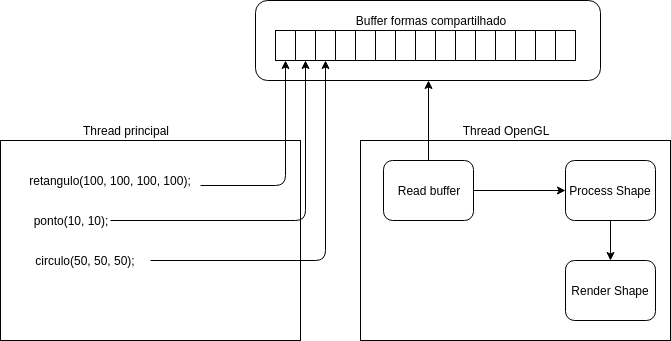
\includegraphics[scale=0.7]{images/basic_architecture.png}
  \caption{Arquitetura proposta}
  \label{fig:arquitetura_proposta}
\end{figure}

A biblioteca gráfica dispõe da API abaixo:

\begin{itemize}
    \item void inicializarBiblioteca(int largura, int altura)
    \item void limparTela()
    
    \item void desfazerUltimaForma()
    \item void refazerUltimaForma()
    
    \item void definirCor(int vermelho, int verde, int azul)
    \item int* obterCor()
    
    \item void definirTamanho(int tamanho)
    \item int obterTamanho()

    \item void poligono(int numeroDeVertices, GLfloat* posicoes)
    \item void ponto(int posX, int posY)
    \item void triangulo(int posX1, int posY1, int posX2, int posY2, int posX3, int posY3)
    \item void retangulo(int posX, int posY, int largura, int altura)
    \item void quadrado(int posX, int posY, int tamanhoLado)
    \item void poligonoRegular(int posX, int posY, int raio, int faces)
    \item void circulo(int posX, int posY, int raio)
    \item void pentagono(int posX, int posY, int raio)
    \item void hexagono(int posX, int posY, int raio)
    \item void decagono(int posX, int posY, int raio)
    \item void dodecagono(int posX, int posY, int raio)
    \item void linha(int posX1, int posY1, int posX2, int posY2)
    
    \item void pausar(int time)
\end{itemize}

\subsubsection{Iniciando a biblioteca}
Apesar de não ter que gerenciar diretamente a janela e o laço de repetição de renderização do OpenGL manualmente, ainda se faz necessário inicializar a biblioteca manualmente, para disparar a thread secundária, responsável pela renderização das formas, e a criação da janela onde serão renderizadas as formas.

A função que inicializa a biblioteca tem a seguinte assinatura:

\begin{lstlisting}
void inicializarBiblioteca(int largura, int altura);
\end{lstlisting}

Os parâmetros de entrada são:

\begin{itemize}
    \item int largura - A largura do tamanho da janela a ser criada.
    \item int altura - A altura do tamanho da janela a ser criada.
\end{itemize}

O exemplo abaixo mostra como inicializar a biblioteca em uma aplicação C:
\begin{lstlisting}
#include <stdio.h>
#include <graphics.h>

int main(void) {
    inicializarBiblioteca(800, 600);
    
    return 0;
}
\end{lstlisting}

\begin{figure}[!htbp]
  \centering
  \includegraphics[scale=0.7]{images/exemplo_initWindow.JPG}
  \caption{Exemplo inicialização da biblioteca}
  \label{fig:exemplo_initWindow}
\end{figure}

\subsubsection{Limpando a tela}
A biblioteca descrita neste trabalho permite que a janela seja limpa, removendo assim todas as formas e reiniciando a janela para seu estado inicial.

A função que limpa a janela tem a seguinte assinatura:

\begin{lstlisting}
void limparTela();
\end{lstlisting}

O exemplo abaixo mostra como limpar a janela em uma aplicação C:

\begin{lstlisting}
#include <stdio.h>
#include "headers/graphics.h"

int main() {
    inicializarBiblioteca(800, 600);

    retangulo(0, 0, 200, 100);
    limparTela();

    getchar();
    return 0;
}
\end{lstlisting}

\subsubsection{Desfazer último desenho}
Em uma aplicação é comum se arrepender de sua última ação e portanto, desfaze-la. A biblioteca aqui implementada possui uma função específica para esta ação. Ela pode ser utilizada múltiplas vezes e a cada vez um desenho é removido da tela.

A função que desfaz o último desenho tem a seguinte assinatura:

\begin{lstlisting}
void desfazerUltimaForma();
\end{lstlisting}

O exemplo abaixo mostra como desfazer o último desenho em uma aplicação C:

\begin{lstlisting}
#include <stdio.h>
#include "headers/graphics.h"

int main() {
    inicializarBiblioteca(800, 600);

    retangulo(0, 0, 200, 100);
    
    definirTamanho(20);
    ponto(50, 50);
    
    desfazerUltimaForma();

    getchar();
    return 0;
}
\end{lstlisting}

\subsubsection{Refazer o último desenho}
Refazer o último desenho é uma opção da mesma forma que desfazer o último desenho, você pode se arrepender e desfazer a opção de desfazer. A cada vez que a função for chamada, um desenho será restaurado. A ordem de restauração é baseada na estrutura de dados pilha, portanto a última forma removida será a primeira forma restaurada. Essa função só pode ser executa caso invocada imediatamente após a função de desfazer, pois caso seja feito um desenho após as opções de desfazer o último desenho, a pilha de ações será descartada.

A função que refaz o último desenho tem a seguinte assinatura:

\begin{lstlisting}
void refazerUltimaForma();
\end{lstlisting}

O exemplo abaixo mostra como refazer o último desenho em uma aplicação C:

\begin{lstlisting}
#include <stdio.h>
#include "headers/graphics.h"

int main() {
    inicializarBiblioteca(800, 600);

    retangulo(0, 0, 200, 100);
    
    definirTamanho(20);
    ponto(50, 50);

    desfazerUltimaForma();
    refazerUltimaForma();

    getchar();
    return 0;
}
\end{lstlisting}

\subsubsection{Alterado a cor de uma forma}
A grande maioria, senão todas, as biblioteca citadas nos trabalhos correlatos permitem a colorização das formas a serem desenhadas.

A função que permite alterar a cor de uma forma tem a seguinte assinatura:

\begin{lstlisting}
void definirCor(int vermelho, int verde, int azul);
\end{lstlisting}

Os parâmetros de entrada são:

\begin{itemize}
    \item int vermelho - Um inteiro de 0 a 255 representando a tonalidade de vermelho do padrão RGB.
    \item int verde - Um inteiro de 0 a 255 representando a tonalidade de verde do padrão RGB.
    \item int azul - Um inteiro de 0 a 255 representando a tonalidade de azul do padrão RGB.
\end{itemize}

O exemplo abaixo mostra como alterar a code de uma forma em uma aplicação C:

\begin{lstlisting}
#include <stdio.h>
#include "headers/graphics.h"

int main() {
    inicializarBiblioteca(800, 600);

    definirCor(255, 0, 127);
    retangulo(0, 0, 200, 100);

    getchar();
    return 0;
}
\end{lstlisting}

\subsubsection{Obter a cor da forma}
Assim como podemos definir a cor de uma forma, também podemos obter sua cor atual. Esta função se faz útil quando, por exemplo, queremos criar uma forma de uma nova cor mas queremos manter a cor antiga porém não é conhecido a cor atual da forma. Como a função \textit{definirCor} recebe 3 argumentos de entrada, a saída é um ponteiro representando um array de inteiros de tamanho 3.

A função que obtém a cor atual de uma forma tem a seguinte assinatura:

\begin{lstlisting}
int* obterCor();
\end{lstlisting}

O exemplo abaixo mostra como obter a cor atual de uma forma em uma aplicação C:

\begin{lstlisting}
#include <stdio.h>
#include "headers/graphics.h"

int main() {
    inicializarBiblioteca(800, 600);

    definirCor(255, 0, 127);
    retangulo(0, 0, 200, 100);

    int* corAtual = obterCor();

    getchar();
    return 0;
}
\end{lstlisting}

\subsubsection{Definindo o tamanho de uma forma}
Algumas formas podem ter seu tamanho alterado. Atualmente apenas a forma \textit{linha(int posX, int posY)} pode ter seu tamanho alterado. Para que surta efeito, \textit{definirTamanho(int tamanho)} deve ser invocada anteriormente a função de desenhar a forma. Após chamado o método de definir o tamanho de uma forma, todas as formas desenhadas após a chamada serão desenhadas com o tamanho definido.

A função que define o tamanho de uma forma tem a seguinte assinatura:

\begin{lstlisting}
void definirTamanho(int tamanho);
\end{lstlisting}

O exemplo abaixo mostra como definir o tamanho de uma forma em uma aplicação C:

\begin{lstlisting}
#include <stdio.h>
#include "headers/graphics.h"

int main() {
    inicializarBiblioteca(800, 600);

    definirTamanho(50);
    ponto(100, 100);

    getchar();
    return 0;
}
\end{lstlisting}

\subsubsection{Obtendo o tamanho de uma forma}
Da mesma forma que é possível definir o tamanho de uma forma, esta API permite que se obtenha o valor atual do tamanho de desenho de formas. Esta função é útil quando você quer desenhar uma forma em novo tamanho porém deseja retornar ao tamanho anterior porém você não possui o conhecimento de qual o valor atual do tamanho da forma.

A função que como obter o tamanho atual de uma forma tem a seguinte assinatura:

\begin{lstlisting}
int obterTamanho();
\end{lstlisting}

O exemplo abaixo mostra como obter o tamanho atual de uma forma em uma aplicação C:

\begin{lstlisting}
#include <stdio.h>
#include "headers/graphics.h"

int main() {
    inicializarBiblioteca(800, 600);

    definirTamanho(50);
    ponto(100, 100);

    int tamanhoAtual = obterTamanho();

    getchar();
    return 0;
}
\end{lstlisting}

\subsubsection{Desenhando um polígono}
Um polígono é uma figura composta por 3 ou mais vértices. A biblioteca permite desenhar polígonos de forma forma livre.

A função que desenha um polígono tem a seguinte assinatura:

\begin{lstlisting}
void poligono(int numeroDeVertices, GLfloat* posicoes);
\end{lstlisting}

Os parâmetros de entrada são:

\begin{itemize}
    \item int numeroDeVertices - Número de vértices que o seu polígono possui
    \item GLfloat* posicoes - Um array contendo as posições de cada vértice.
\end{itemize}

O exemplo abaixo mostra como desenhas um polígono em uma aplicação C:

\begin{lstlisting}
#include <stdio.h>
#include <stdlib.h>
#include "headers/graphics.h"

int main() {
    inicializarBiblioteca(800, 600);

    GLfloat vertices[] = {
        320, 100,
        400, 300,
        800, 50,
        520, 10,
        340, 40
    };
    poligono(5, vertices);

    getchar();
    return 0;
}
\end{lstlisting}

\subsubsection{Desenhando um ponto}
A biblioteca permite que seja desenhado um ponto. O ponto pode ter seu tamanho alterado mediante da função \textit{void definirTamanho(int tamanho);} e por padrão possui o tamanho de 1 pixel.

A função que desenha um pixel tem a seguinte assinatura:

\begin{lstlisting}
void ponto(int posX, int posY);
\end{lstlisting}

Os parâmetros de entrada são:

\begin{itemize}
    \item int posX - A posição X onde o ponto será desenhado.
    \item int posY - A posição Y onde o ponto será desenhado.
\end{itemize}

O exemplo abaixo mostra como desenhar um ponto com tamanho 20 em uma aplicação C:

\begin{lstlisting}
#include <stdio.h>
#include <stdlib.h>
#include "headers/graphics.h"

int main() {
    inicializarBiblioteca(800, 600);

    definirTamanho(20);
    poligono(10, 10);

    getchar();
    return 0;
}
\end{lstlisting}

\subsubsection{Desenhando um triângulo}
Em uma biblioteca gráfica, triângulos são uma das formas mais básicas e utilizadas, pois todos os polígonos convexo pode ser decomposto em vários triângulos.

A função que desenha um triângulo tem a seguinte assinatura:

\begin{lstlisting}
void triangulo(int posX1, int posY1, int posX2, int posY2, int posX3, int posY3);
\end{lstlisting}

Os parâmetros de entrada são:

\begin{itemize}
    \item int posX1 - Posição X da vértice 1 de onde o triângulo será desenhado.
    \item int posY1 - Posição Y da vértice 1 de onde o triângulo será desenhado.

    \item int posX2 - Posição X da vértice 2 de onde o triângulo será desenhado.
    \item int posY2 - Posição Y da vértice 2 de onde o triângulo será desenhado.

    \item int posX3 - Posição X da vértice 3 de onde o triângulo será desenhado.
    \item int posY3 - Posição Y da vértice 3 de onde o triângulo será desenhado.
\end{itemize}

O exemplo abaixo mostra como desenhar um triângulo em uma aplicação C:

\begin{lstlisting}
#include <stdio.h>
#include <stdlib.h>
#include "headers/graphics.h"

int main() {
    inicializarBiblioteca(800, 600);

    triangulo(
        100, 100,
        300, 100,
        200, 300
    );

    getchar();
    return 0;
}
\end{lstlisting}

\subsubsection{Desenhando um retângulo}
Retângulos são formas que possuem 4 ângulos retos e também são bastante utilizados para desenhos além de ser uma das formas mais básicas.

A função que desenha um retângulo tem a seguinte assinatura:

\begin{lstlisting}
void retangulo(int posX, int posY, int largura, int altura);
\end{lstlisting}

Os parâmetros de entrada são:

\begin{itemize}
    \item int posX - Posição X onde o retângulo será desenhado. Representa o vértice inferior esquerdo do retângulo.
    \item int posY - Posição y onde o retângulo será desenhado. Representa o vértice inferior esquerdo do retângulo.
    \item int altura - Altura do triângulo.
    \item int largura - Largura do triângulo.
\end{itemize}

O exemplo abaixo mostra como criar um triângulo em uma aplicação C:

\begin{lstlisting}
#include <stdio.h>
#include <stdlib.h>
#include "headers/graphics.h"

int main() {
    inicializarBiblioteca(800, 600);

    retangulo(100, 100, 200, 300);

    getchar();
    return 0;
}
\end{lstlisting}

\subsubsection{Desenhando um quadrado}
Um quadrado é um polígono considerado especial, pois ele é um retângulo onde tanto a altura quanto a largura são iguais.

A função que desenha um quadrado tem a seguinte assinatura:

\begin{lstlisting}
void quadrado(int posX, int posY, int tamanhoLado);
\end{lstlisting}

Os parâmetros de entrada são:

\begin{itemize}
    \item int posX - Posição X onde o quadrado será desenhado. Representa o vértice inferior esquerdo do quadrado.
    \item int posY - Posição Y onde o quadrado será desenhado. Representa o vértice inferior esquerdo do quadrado.
    \item int tamanhoLado - Representa o valor do lado do quadrado. Será tanto a altura quanto a largura desta forma.
\end{itemize}

O exemplo abaixo mostra como desenhar um quadrado verde em uma aplicação C:

\begin{lstlisting}
#include <stdio.h>
#include <stdlib.h>
#include "headers/graphics.h"

int main() {
    inicializarBiblioteca(800, 600);

    definirCor(0, 255, 0);
    quadrado(100, 100, 200);

    getchar();
    return 0;
}
\end{lstlisting}

\subsubsection{Desenhando um polígono regular}
Um polígono regular é um polígono convexo com \textit{n} faces onde cada face possui o mesmo tamanho e todos os ângulos internos são iguais.

A função que desenha um polígono regular tem a seguinte assinatura:

\begin{lstlisting}
void poligonoRegular(int posX, int posY, int raio, int faces);
\end{lstlisting}

Os parâmetros de entrada são:

\begin{itemize}
    \item int posX - Posição X onde o polígono será desenhado. Representa o centro de onde será desenhado o polígono regular.
    \item int posY - Posição Y onde o polígono será desenhado. Representa o centro de onde será desenhado o polígono regular.
    \item int raio - Tamanho do raio que o polígono regular possuirá.
    \item int faces - O número de faces que o polígono regular possuirá.
\end{itemize}

O exemplo abaixo mostra como desenhar um polígono regular azul em uma aplicação C:

\begin{lstlisting}
#include <stdio.h>
#include <stdlib.h>
#include "headers/graphics.h"

int main() {
    inicializarBiblioteca(800, 600);

    definirCor(0, 0, 255);
    poligonoRegular(300, 300, 100, 7);

    getchar();
    return 0;
}
\end{lstlisting}

\subsubsection{Desenhando um círculo}
O círculo é uma forma geométrica que possui virtualmente infinitos vértices.
A função que [DESCREVER_FUNCAO] tem a seguinte assinatura:

\begin{lstlisting}
[ASSINATURA_FUNCAO]
\end{lstlisting}

Os parâmetros de entrada são:

\begin{itemize}
    \item int p1 - Parâmetro 1
    \item int p2 - Parâmetro 2
    \item const char* p3 - Parâmetro 3
\end{itemize}

O exemplo abaixo mostra como [DESCREVER_FUNCAO] em uma aplicação C:

\begin{lstlisting}
[CODIGO_EXEMPLO_FUNCAO]
\end{lstlisting}

\subsubsection{void pentagono(int posX, int posY, int raio)}
[DESCRICAO]
A função que [DESCREVER_FUNCAO] tem a seguinte assinatura:

\begin{lstlisting}
[ASSINATURA_FUNCAO]
\end{lstlisting}

Os parâmetros de entrada são:

\begin{itemize}
    \item int p1 - Parâmetro 1
    \item int p2 - Parâmetro 2
    \item const char* p3 - Parâmetro 3
\end{itemize}

O exemplo abaixo mostra como [DESCREVER_FUNCAO] em uma aplicação C:

\begin{lstlisting}
[CODIGO_EXEMPLO_FUNCAO]
\end{lstlisting}

\subsubsection{void hexagono(int posX, int posY, int raio)}
[DESCRICAO]
A função que [DESCREVER_FUNCAO] tem a seguinte assinatura:

\begin{lstlisting}
[ASSINATURA_FUNCAO]
\end{lstlisting}

Os parâmetros de entrada são:

\begin{itemize}
    \item int p1 - Parâmetro 1
    \item int p2 - Parâmetro 2
    \item const char* p3 - Parâmetro 3
\end{itemize}

O exemplo abaixo mostra como [DESCREVER_FUNCAO] em uma aplicação C:

\begin{lstlisting}
[CODIGO_EXEMPLO_FUNCAO]
\end{lstlisting}

\subsubsection{void decagono(int posX, int posY, int raio)}
[DESCRICAO]
A função que [DESCREVER_FUNCAO] tem a seguinte assinatura:

\begin{lstlisting}
[ASSINATURA_FUNCAO]
\end{lstlisting}

Os parâmetros de entrada são:

\begin{itemize}
    \item int p1 - Parâmetro 1
    \item int p2 - Parâmetro 2
    \item const char* p3 - Parâmetro 3
\end{itemize}

O exemplo abaixo mostra como [DESCREVER_FUNCAO] em uma aplicação C:

\begin{lstlisting}
[CODIGO_EXEMPLO_FUNCAO]
\end{lstlisting}

\subsubsection{void dodecagono(int posX, int posY, int raio)}
[DESCRICAO]
A função que [DESCREVER_FUNCAO] tem a seguinte assinatura:

\begin{lstlisting}
[ASSINATURA_FUNCAO]
\end{lstlisting}

Os parâmetros de entrada são:

\begin{itemize}
    \item int p1 - Parâmetro 1
    \item int p2 - Parâmetro 2
    \item const char* p3 - Parâmetro 3
\end{itemize}

O exemplo abaixo mostra como [DESCREVER_FUNCAO] em uma aplicação C:

\begin{lstlisting}
[CODIGO_EXEMPLO_FUNCAO]
\end{lstlisting}

\subsubsection{void linha(int posX1, int posY1, int posX2, int posY2)}
[DESCRICAO]
A função que [DESCREVER_FUNCAO] tem a seguinte assinatura:

\begin{lstlisting}
[ASSINATURA_FUNCAO]
\end{lstlisting}

Os parâmetros de entrada são:

\begin{itemize}
    \item int p1 - Parâmetro 1
    \item int p2 - Parâmetro 2
    \item const char* p3 - Parâmetro 3
\end{itemize}

O exemplo abaixo mostra como [DESCREVER_FUNCAO] em uma aplicação C:

\begin{lstlisting}
[CODIGO_EXEMPLO_FUNCAO]
\end{lstlisting}


\subsubsection{void pausar(int time)}
A função que [DESCREVER_FUNCAO] tem a seguinte assinatura:

\begin{lstlisting}
[ASSINATURA_FUNCAO]
\end{lstlisting}

O exemplo abaixo mostra como [DESCREVER_FUNCAO] em uma aplicação C:

\begin{lstlisting}
[CODIGO_EXEMPLO_FUNCAO]
\end{lstlisting}



\subsection{Exemplos de Uso}

\subsection{Documentação}

\section{Estado Atual do Desenvolvimento}
Estado Atual

\section{Trabalhos Futuros}
Trabalhos Futuros

\chapter{Considerações Finais}

\section{Dificuldades Encontradas}

\begin{itemize}
  
  \item Compilar multi plataforma
  \item Instalação da biblioteca GLFW
  \item Corrupção da memória HEAP no Windows
  \item Instalação da biblioteca no Code::Blocks
  
\end{itemize}

\section{Conclusão}
Conclusão

%\chapter{Desenvolvimento}
%Um ou mais capítulos (por exemplo um para testes)

% ---
% Conclusão
% ---
\iffalse
\chapter*[Conclusão]{Conclusão}
\addcontentsline{toc}{chapter}{Conclusão}
%TCC:
Descrever aqui as conclusões e/ou considerações finais.
Destacar as contribuições originais do trabalho.
Propor trabalhos futuros em continuidade ao trabalho realizado.
\fi

% ----------------------------------------------------------
% ELEMENTOS PÓS-TEXTUAIS
% ----------------------------------------------------------
\postextual

%\nocite{babel}
% ----------------------------------------------------------
% Referências bibliográficas
% ----------------------------------------------------------
\bibliography{referencias}


%% ----------------------------------------------------------
%% Apêndices TCC: só mantenha se for pertinente.
%% ----------------------------------------------------------

\iffalse
% ---
% Inicia os apêndices
% ---
\begin{apendicesenv}

% Imprime uma página indicando o início dos apêndices
\partapendices
% ----------------------------------------------------------
\chapter{Quisque libero justo}
% ----------------------------------------------------------

\lipsum[50]

% ----------------------------------------------------------
\chapter{Coisas que fiz e que achei interessante mas não tanto para entrar no corpo do texto}
% ----------------------------------------------------------
\lipsum[55-57]
\end{apendicesenv}
\fi
% ---


% ----------------------------------------------------------
% Anexos %TCC: so mantenha se pertinente.
% ----------------------------------------------------------

\iffalse
% ---
% Inicia os anexos
% ---
\begin{anexosenv}

% Imprime uma página indicando o início dos anexos
\partanexos
% ---
\chapter{Eu sempre quis aprender latim}
% ---
\lipsum[30]

% ---
\chapter{Coisas que eu não fiz mas que achei interessante o suficiente para colocar aqui}
% ---

\lipsum[31]

% ---
\chapter{Fusce facilisis lacinia dui}
% ---

\lipsum[32]
\end{anexosenv}
\fi

%---------------------------------------------------------------------
% INDICE REMISSIVO
%---------------------------------------------------------------------

\printindex



\end{document}
